\chapter{多重循环分析}

\section{实验目的}
C语言编写多重循环程序(大于3重),查看其反汇编码,分析各条语句功能,并采用汇编语言重写相同功能程序。

\section{程序流程}
\begin{enumerate}
    \item 编写四重循环的C语言代码;
    \item 反汇编分析语句功能;
    \item 重写反汇编代码。
\end{enumerate}

\section{具体实现}
该节部分主要介绍了多重循环的C代码反汇编的分析以及代码的重写。
\subsection{多重循环的C语言代码}
设置四重循环,选取a数组中的四个数相加输出结果,其中为了方便显示不同循环次数,对每一次循环的边界值设定不一致。

具体代码如下:
\begin{lstlisting}
#include<stdio.h>
int a[10] = { 1,2,3,4,5,6,7,8,9 };
int main()
{
    for (int i = 0; i < 2; i++)
    {
        for (int j = 0; j < 3; j++)
        {
            for (int k = 0; k < 4; k++)
            {
                for (int m = 0; m < 5; m++)
                {
                    int sum = a[i] + a[j] + a[k] + a[m];
                    printf("%d\n", sum);
                }
            }
        }
    }
    return 0;
}
\end{lstlisting}

\subsection{反汇编分析}
点击调试后,查看反汇编得到汇编代码,并对语句进行分析。

分析过程如下:
\subsubsection{初始化}
\begin{lstlisting}
    00C61860  push        ebp  
    00C61861  mov         ebp,esp  
    00C61863  sub         esp,0FCh  
    00C61869  push        ebx  
    00C6186A  push        esi  
    00C6186B  push        edi  
    00C6186C  lea         edi,[ebp-0FCh]  
    00C61872  mov         ecx,3Fh  
    00C61877  mov         eax,0CCCCCCCCh  
    00C6187C  rep stos    dword ptr es:[edi]  
    00C6187E  mov         ecx,offset _B5E6F96D_多重循环@cpp (0C6C003h)  
    00C61883  call        @__CheckForDebuggerJustMyCode@4 (0C61316h) 
\end{lstlisting}
{\bfseries 1. push ebp}:将ebp压栈,保存调用函数的栈指针。
\\{\bfseries 2. mov ebp,esp}:把esp的值赋给ebp,也就是ebp指向栈基址
\\{\bfseries 3. sub esp,0FCh}:为当前函数开辟局部变量空间
\\{\bfseries 4. push ebx}
\\{\bfseries 5. push esi}
\\{\bfseries 6. push edi}:将ebx、esi、edi的值保存下来(压入栈中)
\\{\bfseries 7. lea edi,[ebp-0FCh]}:取出栈中局部变量区域(大小为0FCh=252的那一块)的最低地址
\\{\bfseries 8. mov ecx,3Fh}:把63赋给ecx
\\{\bfseries 9. mov eax,0CCCCCCCCh}:把0CCCCCCCCh赋给eax
\\{\bfseries 10. rep stos dword ptr es:[edi]}:将局部变量区域全部初始化为0CCCCCCCCh(这里63*4=252)

\subsubsection{内部循环体}
\begin{lstlisting}
	for (int i = 0; i < 2; i++)
;i=0
00C61888  mov         dword ptr [ebp-8],0  
00C6188F  jmp         main+3Ah (0C6189Ah)  
00C61891  mov         eax,dword ptr [ebp-8]  
00C61894  add         eax,1  
00C61897  mov         dword ptr [ebp-8],eax
;判断i是否<2  
00C6189A  cmp         dword ptr [ebp-8],2  
;如果不小于,跳出循环
00C6189E  jge         main+0D6h (0C61936h)  
	{
		for (int j = 0; j < 3; j++)
;j=0
00C618A4  mov         dword ptr [ebp-14h],0  
00C618AB  jmp         main+56h (0C618B6h)  
00C618AD  mov         eax,dword ptr [ebp-14h]  
00C618B0  add         eax,1  
00C618B3  mov         dword ptr [ebp-14h],eax 
;j<3? 
00C618B6  cmp         dword ptr [ebp-14h],3  
;跳到i的循环体里
00C618BA  jge         main+0D1h (0C61931h)  
		{
			for (int k = 0; k < 4; k++)
;k=0
00C618BC  mov         dword ptr [ebp-20h],0  
00C618C3  jmp         main+6Eh (0C618CEh)  
00C618C5  mov         eax,dword ptr [ebp-20h]  
00C618C8  add         eax,1  
00C618CB  mov         dword ptr [ebp-20h],eax  
;k<4?
00C618CE  cmp         dword ptr [ebp-20h],4  
跳到j的循环里
00C618D2  jge         main+0CCh (0C6192Ch)  
			{
				for (int m = 0; m < 5; m++)
00C618D4  mov         dword ptr [ebp-2Ch],0  
00C618DB  jmp         main+86h (0C618E6h)  
00C618DD  mov         eax,dword ptr [ebp-2Ch]  
00C618E0  add         eax,1  
00C618E3  mov         dword ptr [ebp-2Ch],eax  
00C618E6  cmp         dword ptr [ebp-2Ch],5 
;跳到k的循环里 
00C618EA  jge         main+0CAh (0C6192Ah)  
                    {
int sum = a[i] + a[j] + a[k] + a[m];
;取出a数组对应的值
00C618EC  mov         eax,dword ptr [ebp-8]  
00C618EF  mov         ecx,dword ptr a (0C6A000h)[eax*4]  
00C618F6  mov         edx,dword ptr [ebp-14h]  
00C618F9  add         ecx,dword ptr a (0C6A000h)[edx*4]  
00C61900  mov         eax,dword ptr [ebp-20h]  
00C61903  add         ecx,dword ptr a (0C6A000h)[eax*4]  
00C6190A  mov         edx,dword ptr [ebp-2Ch]  
00C6190D  add         ecx,dword ptr a (0C6A000h)[edx*4]  
00C61914  mov         dword ptr [ebp-38h],ecx  
					printf("%d\n", sum);
00C61917  mov         eax,dword ptr [ebp-38h]  
00C6191A  push        eax  
00C6191B  push        offset string "%d\n" (0C67B30h)  
00C61920  call        _printf (0C610CDh)  
;平衡堆栈
00C61925  add         esp,8  
				}
00C61928  jmp         main+7Dh (0C618DDh)  
			}
00C6192A  jmp         main+65h (0C618C5h)  
		}
00C6192C  jmp         main+4Dh (0C618ADh)  
	}
00C61931  jmp         main+31h (0C61891h)  
	return 0;
00C61936  xor         eax,eax  
}
\end{lstlisting}
根据上图展示的汇编代码以及相关注释,可以得到多重循环的逻辑结构。
\begin{figure}[H]
    \centering
    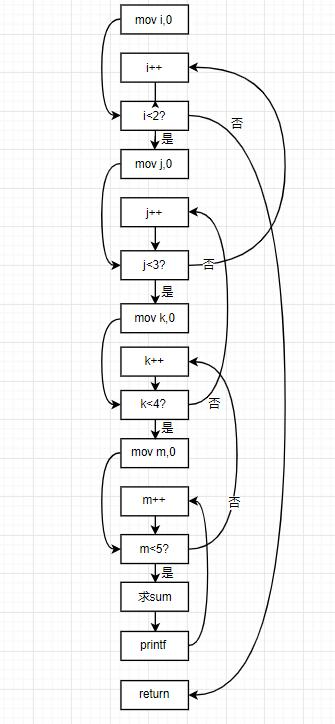
\includegraphics[width= 0.55\textwidth]{assets/多重循环}
    \caption{多重循环分析}
    \label{多重循环分析}
\end{figure}

\subsection{重写多重循环}
根据上述的代码逻辑结构,重写汇编程序如下:
\begin{lstlisting}
main proc
	local @i:dword,@j:dword,@k:dword,@m:dword,@sum:dword
	mov @i,0
	jmp L1
L4:
	add @i,1
L1:
	cmp @i,2
	jge L2
	mov @j,0
	jmp L3
L6:
	add @j,1
L3:
	cmp @j,3
	jge L4
	mov @k,0
	jmp L5
L8:
	add @k,1
L5:
	cmp @k,4
	jge L6
	mov @m,0
	jmp L7
L9:
	add @m,1
L7:
	cmp @m,5
	jge L8
	;计算sum
	mov eax,@i
	mov ecx,a[eax*4]
	mov eax,@j
	add ecx,a[eax*4]
	mov eax,@k
	add ecx,a[eax*4]
	mov eax,@m
	add ecx,a[eax*4]
	mov @sum,ecx
	;输出结果
	invoke printf,offset printStrlen,@sum
	jmp L9
L2:
	ret
	
main endp
end main
\end{lstlisting}
\section{实验结果展示}

% \subsection{两个文件相同}
\begin{figure}[H]
    \centering
    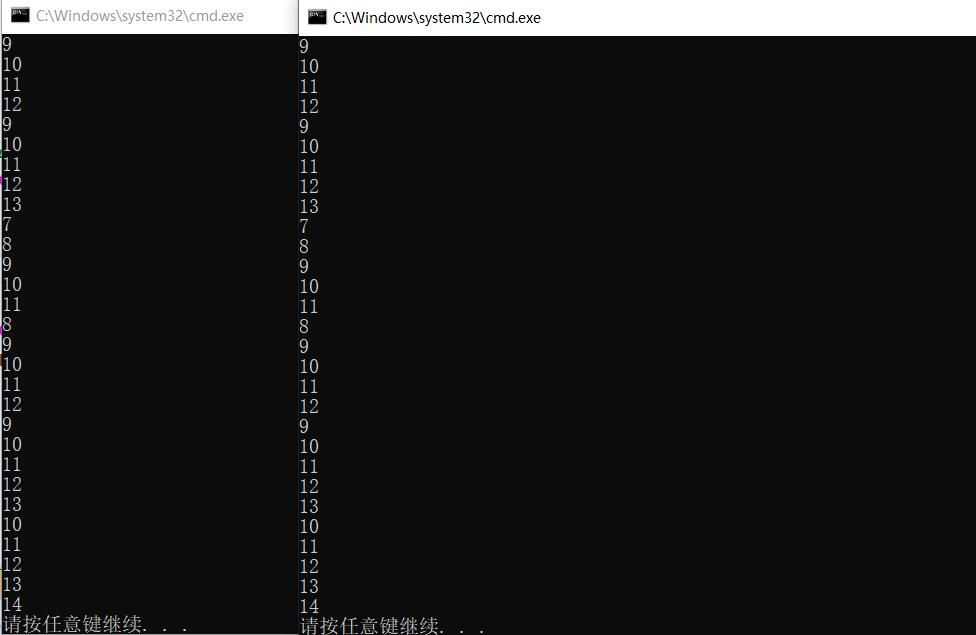
\includegraphics[width= 0.9\textwidth]{assets/多重循环结果}
    \caption{多重循环结果}
    \label{多重循环结果}
\end{figure}

% \subsection{两个文件内容不同}
% \begin{figure}[H]
%     \centering
%     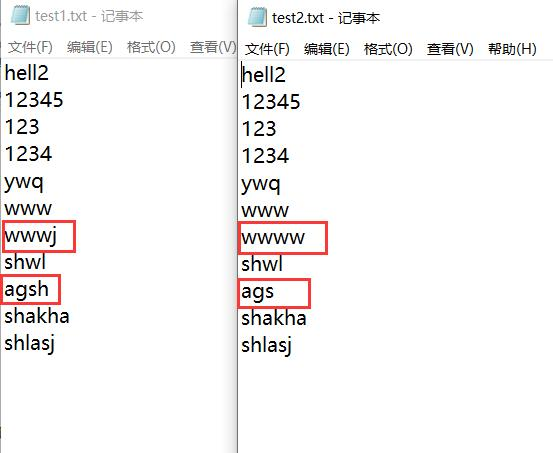
\includegraphics[width= 0.9\textwidth]{assets/文件比对2}
%     \caption{文件内容不同}
%     \label{文件内容不同}
% \end{figure}
% \begin{figure}[H]
%     \centering
%     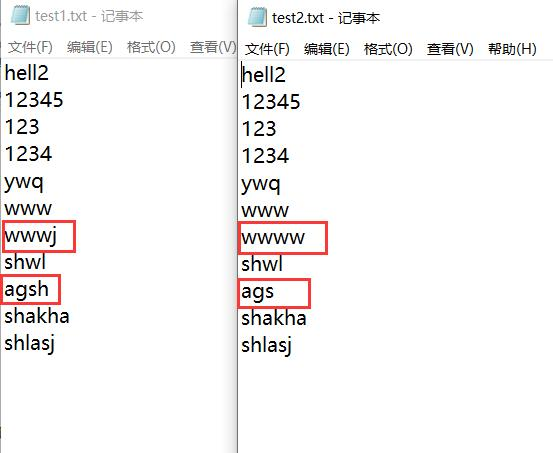
\includegraphics[width= 0.9\textwidth]{assets/文件比对2}
%     \caption{文件比对结果}
%     \label{文件比对结果2}
% \end{figure}

